\textbf{信号:}数据的电气或电磁的表现(就是将数据用另外一种形态表现出来,就好像水转换成冰,其实质还是水,仅仅是形态变了)。而数据是传送信息(如图片和文字等)的实体。

{\textbf{注意1:}}无论数据或信号,都既可以是模拟的,也可以是数字的。``模拟的''就是连续变化的,如图2-1所示;而``数字的''表示取值仅允许是有限的离散值,如图2-2所示。

{\textbf{注意2:}}信道上传送的信号分为\textbf{基带信号和宽带信号}。基带信号是将数字信号0和1直接用两种不同的电压表示,然后传送到数字信道上去传输,称为基带传输;宽带信号是将基带信号进行调制后形成模拟信号,然后再传送到模拟信道上去传输,称为宽带传输。总之,记住一句话:{基带对应数字信号,宽带对应模拟信号。}

{\textbf{注意3:}}宽带传输在考研中可以等同于频带传输(都是传输模拟信号),只是宽带传输比频带传输有更多的子信道,并且这些子信道都可以同时发送信号。

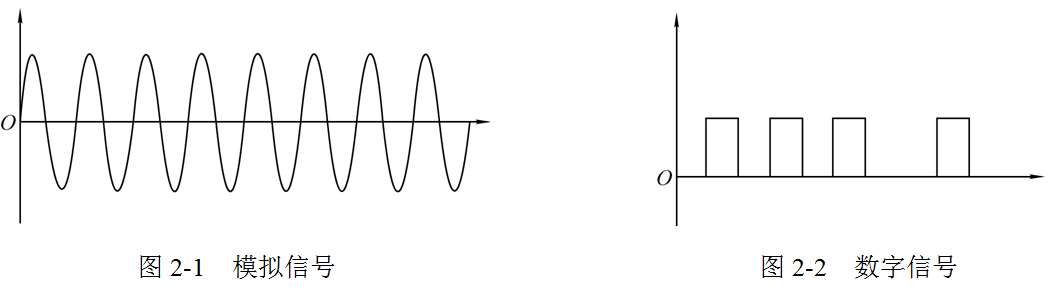
\includegraphics[width=6in]{png-jpeg-pics/49645200BFF6E52CA9164749D488B84B.png}
